\documentclass[12pt,a4paper,openright,twoside]{book}
\usepackage[utf8]{inputenc}
\usepackage{disi-thesis}
\usepackage{code-lstlistings}
\usepackage{notes}
\usepackage{shortcuts}
\usepackage{acronym}
\usepackage{hyperref}
\usepackage{biblatex}
\usepackage{changepage}
\usepackage[acronym]{glossaries}
\addbibresource{bibliography.bib}

\school{\unibo}
\programme{Corso di Laurea in Ingegneria e Scienze Informatiche}
\title{Sviluppo di un sistema di visione artificiale per la rilevazione e la stima della posa basata su marker ArUco in Java}
\author{Bacchini Lorenzo}
\date{\today}
\subject{Programmazione ad oggetti}
\supervisor{Prof. Mirko Viroli}
\cosupervisor{Dott. Gianluca Aguzzi}
\session{III}
\academicyear{2023-2024}

% Definition of acronyms
%\acrodef{IoT}{Internet of Thing}
%\acrodef{vm}[VM]{Virtual Machine}


\mainlinespacing{1.241} % line spacing in mainmatter, comment to default (1)
\makeglossaries
\newglossaryentry{FullHD}
{
	name=FullHD,
	description={risoluzione di 1920 x 1080 pixel}
} 
\newglossaryentry{nodi}
{
	name=nodi,
	description=dispositivi visti come elementi di una rete
}
\newglossaryentry{nodo}
{
	name=nodo,
	description=dispositivo visto come elemento di una rete
}
\newglossaryentry{scena}
{
	name=scena,
	description=campo visivo della videocamera
}
\newglossaryentry{dizionario4x4_100}{
	name=DICT\textunderscore4X4\textunderscore100,
	description=dizionario con marker 4x4 e con una quantità massima di marker istanziabili pari a 100
}
\newacronym{ocr}{OCR}{optical character recognition}
\newacronym{aruco}{ArUco}{Augmented Reality University of Cordova}
\newacronym{jvm}{JVM}{Java Virtual Machine}
\newacronym{gui}{GUI}{Graphical User Interface}
\newacronym{opencv}{OpenCV}{Open Source Computer Vision Library}

\begin{document}

\frontmatter\frontispiece

\begin{abstract}	
Max 2000 characters, strict.
\end{abstract}

\begin{dedication} % this is optional
Optional. Max a few lines.
\end{dedication}

%----------------------------------------------------------------------------------------
\tableofcontents   
\listoffigures     % (optional) comment if empty
\lstlistoflistings % (optional) comment if empty
%----------------------------------------------------------------------------------------

\mainmatter

%----------------------------------------------------------------------------------------
\chapter{Introduzione}
questo capitolo lo scriverò alla fine ma devo ricordarmi di dire che il mio contributo al progetto è stato particolare perché in un ambiente outdoor non sarebbe stato necessario l'utilizzo di marker \acrfull{aruco} e camere, ma sarebbe bastato il GPS \label{chap:introduction}
%----------------------------------------------------------------------------------------

Write your intro here.
\sidenote{Add sidenotes in this way. They are named after the author of the thesis}

You can use acronyms that your defined previously,
such as 
%
If you use acronyms twice,
they will be written in full only once
(indeed, you can mention the now without it being fully explained).
%
In some cases, you may need a plural form of the acronym.
%
For instance,
that you are discussing,
you may need both  and .

\paragraph{Structure of the Thesis}

\note{At the end, describe the structure of the paper}

\chapter{Background}

\section{Visione artificiale}

\subsection{Cos'è la visione artificiale?}
Quando parliamo di visione artificiale o computer vision stiamo considerando un insieme di processi e tecniche che hanno come scopo finale quello di trasformare degli input (solitamente foto o video \footnote{gli input potrebbero essere anche generati da scanner, sensori LiDaR, radar ecc.}) in una serie di informazioni utili al calcolatore, che possono poi essere utilizzate per prendere decisioni in maniera autonoma, analizzare una situazione o addirittura creare una rappresentazione del mondo reale 3D che ci circonda. \cite{bradski2008learning} \cite{microsoftArtificialVision}

Quanto sopra descritto non è troppo diverso da ciò che i nostri occhi fanno tutti i giorni, ed infatti, la visione artificiale nasce proprio per permettere al calcolatore di ``vedere" esattamente come un essere umano, in modo da poter interagire con l'ambiente circostante.

\subsection{Come funziona la visione artificiale?}
Il processo di visione artificiale può essere suddiviso tre fasi principali:
\begin{enumerate}
	\item Acquisizione di un'immagine
	\item Interpretazione e analisi dell'immagine
	\item Richiesta di informazioni sull'immagine analizzata
\end{enumerate}
Nella fase di rilevazione come sopra citato è possibile utilizzare diversi tipi di strumenti come fotocamere o videocamere, ma è nella fase centrale che il processo può differire maggiormente, infatti, l'interpretazione dell'immagine viene effettuata secondo algoritmi che possono essere anche molto diversi in base al loro scopo, negli ultimi anni inoltre si stanno facendo largo nuove tecnologie \footnote{con il termine nuove non si intende che tecnologie come l'intelligenza artificiale o il machine learning siano state sviluppate negli ultimi anni, ma che iniziano ad essere prese sempre più in considerazione nell'ambito della visione artificiale} come l'intelligenza artificiale, il machine learning e il deep learning per poter intraprendere decisioni e svolgere compiti in modo autonomo senza il bisogno dell'intervento umano.

\subsection{Applicazioni e finalità}
Di seguito sono elencate alcune applicazioni della visione artificiale:
\begin{itemize}
	\item Classificazione di immagini
	\item Identificazione di oggetti
	\item Suddivisione di immagini in sezioni da analizzare
	\item Riconoscimento facciale
	\item Rilevazione e riconoscimento dei sentimenti di un soggetto
	\item Ricostruzione di ambienti 3D
	\item Guida autonoma
\end{itemize}
La lista dei possibili utilizzi è ovviamente molto vasta ma quelli riportati sopra sono tra i più gettonati sia in ambito professionale che di ricerca.

\subsection{Principali criticità}
Tutte le operazioni che caratterizzano un sistema di visione artificiale possono essere largamente influenzate da una serie di condizioni interne o esterne con il risultato che il nostro sistema potrebbe non operare come previsto.

Un esempio di condizioni esterne che possono influenzare il comportamento del nostro sistema sono sicuramente l'illuminazione, la prospettiva ed eventuali occlusioni dell'immagine in input, che possono portare ad una maggiore difficoltà di rilevazione e riconoscimento, per quanto riguarda invece i parametri interni possiamo considerare la risoluzione della camera che stiamo utilizzando, l'algoritmo di elaborazione e la complessità (in termini di numero di pixel da elaborare) dell'immagine ottenuta, come parametri che possono variare anche di molto la velocità e la precisione del nostro sistema.

\subsection{Cenni storici}
I primi articoli prodotti riguardanti la visione artificiale risalgono agli anni '60 dove però l'idea di poter acquisire immagini ed elaborarle, facendone comprendere il contenuto all'elaboratore era ancora troppo precoce per l'hardware a disposizione,
solo intorno agli anni '80 si sono iniziati a vedere i primi sviluppi significativi grazie all'introduzione della \href{https://en.wikipedia.org/wiki/Hough_transform}{trasformata di Hough}
e dei primi algoritmi di riconoscimento ottico dei caratteri \acrfull{ocr}.
Dagli anni '90 sino ai primi anni '00 l'attenzione si è spostata sullo sviluppo di algoritmi di machine learning, questo ha permesso nel 2001 di sviluppare il primo algoritmo di riconoscimento facciale.\cite{artificialVisionHistory}

Ad oggi la visione artificiale adotta tecniche e processi completamente differenti rispetto a quelli visti nei suoi primi anni di sviluppo, facendo largo uso di reti convoluzionali e dell'intelligenza artificiale (ormai largamente utilizzabile grazie alla sempre crescente potenza di calcolo a disposizione) che le permettono non solo di essere più veloce ma anche di garantire una precisione dei risultati molto maggiore grazie anche al vasto numero di dati a disposizione.

\section{Marker fiduciari} \label{sec:marker_fiduciari}
I marker fiduciari sono degli oggetti che, posti all'interno del campo visivo di una fotocamera possono essere utilizzati come punti di riferimento. 

Gli scopi principali di questi marker sono sicuramente la calibrazione della camera, la localizzazione, il tracking e la rilevazione di oggetti.

Alcuni possibili tipi di marker fiduciari sono riportati nella figura \ref{fig:marker_fiduciari}:

\begin{figure}
	\centering
	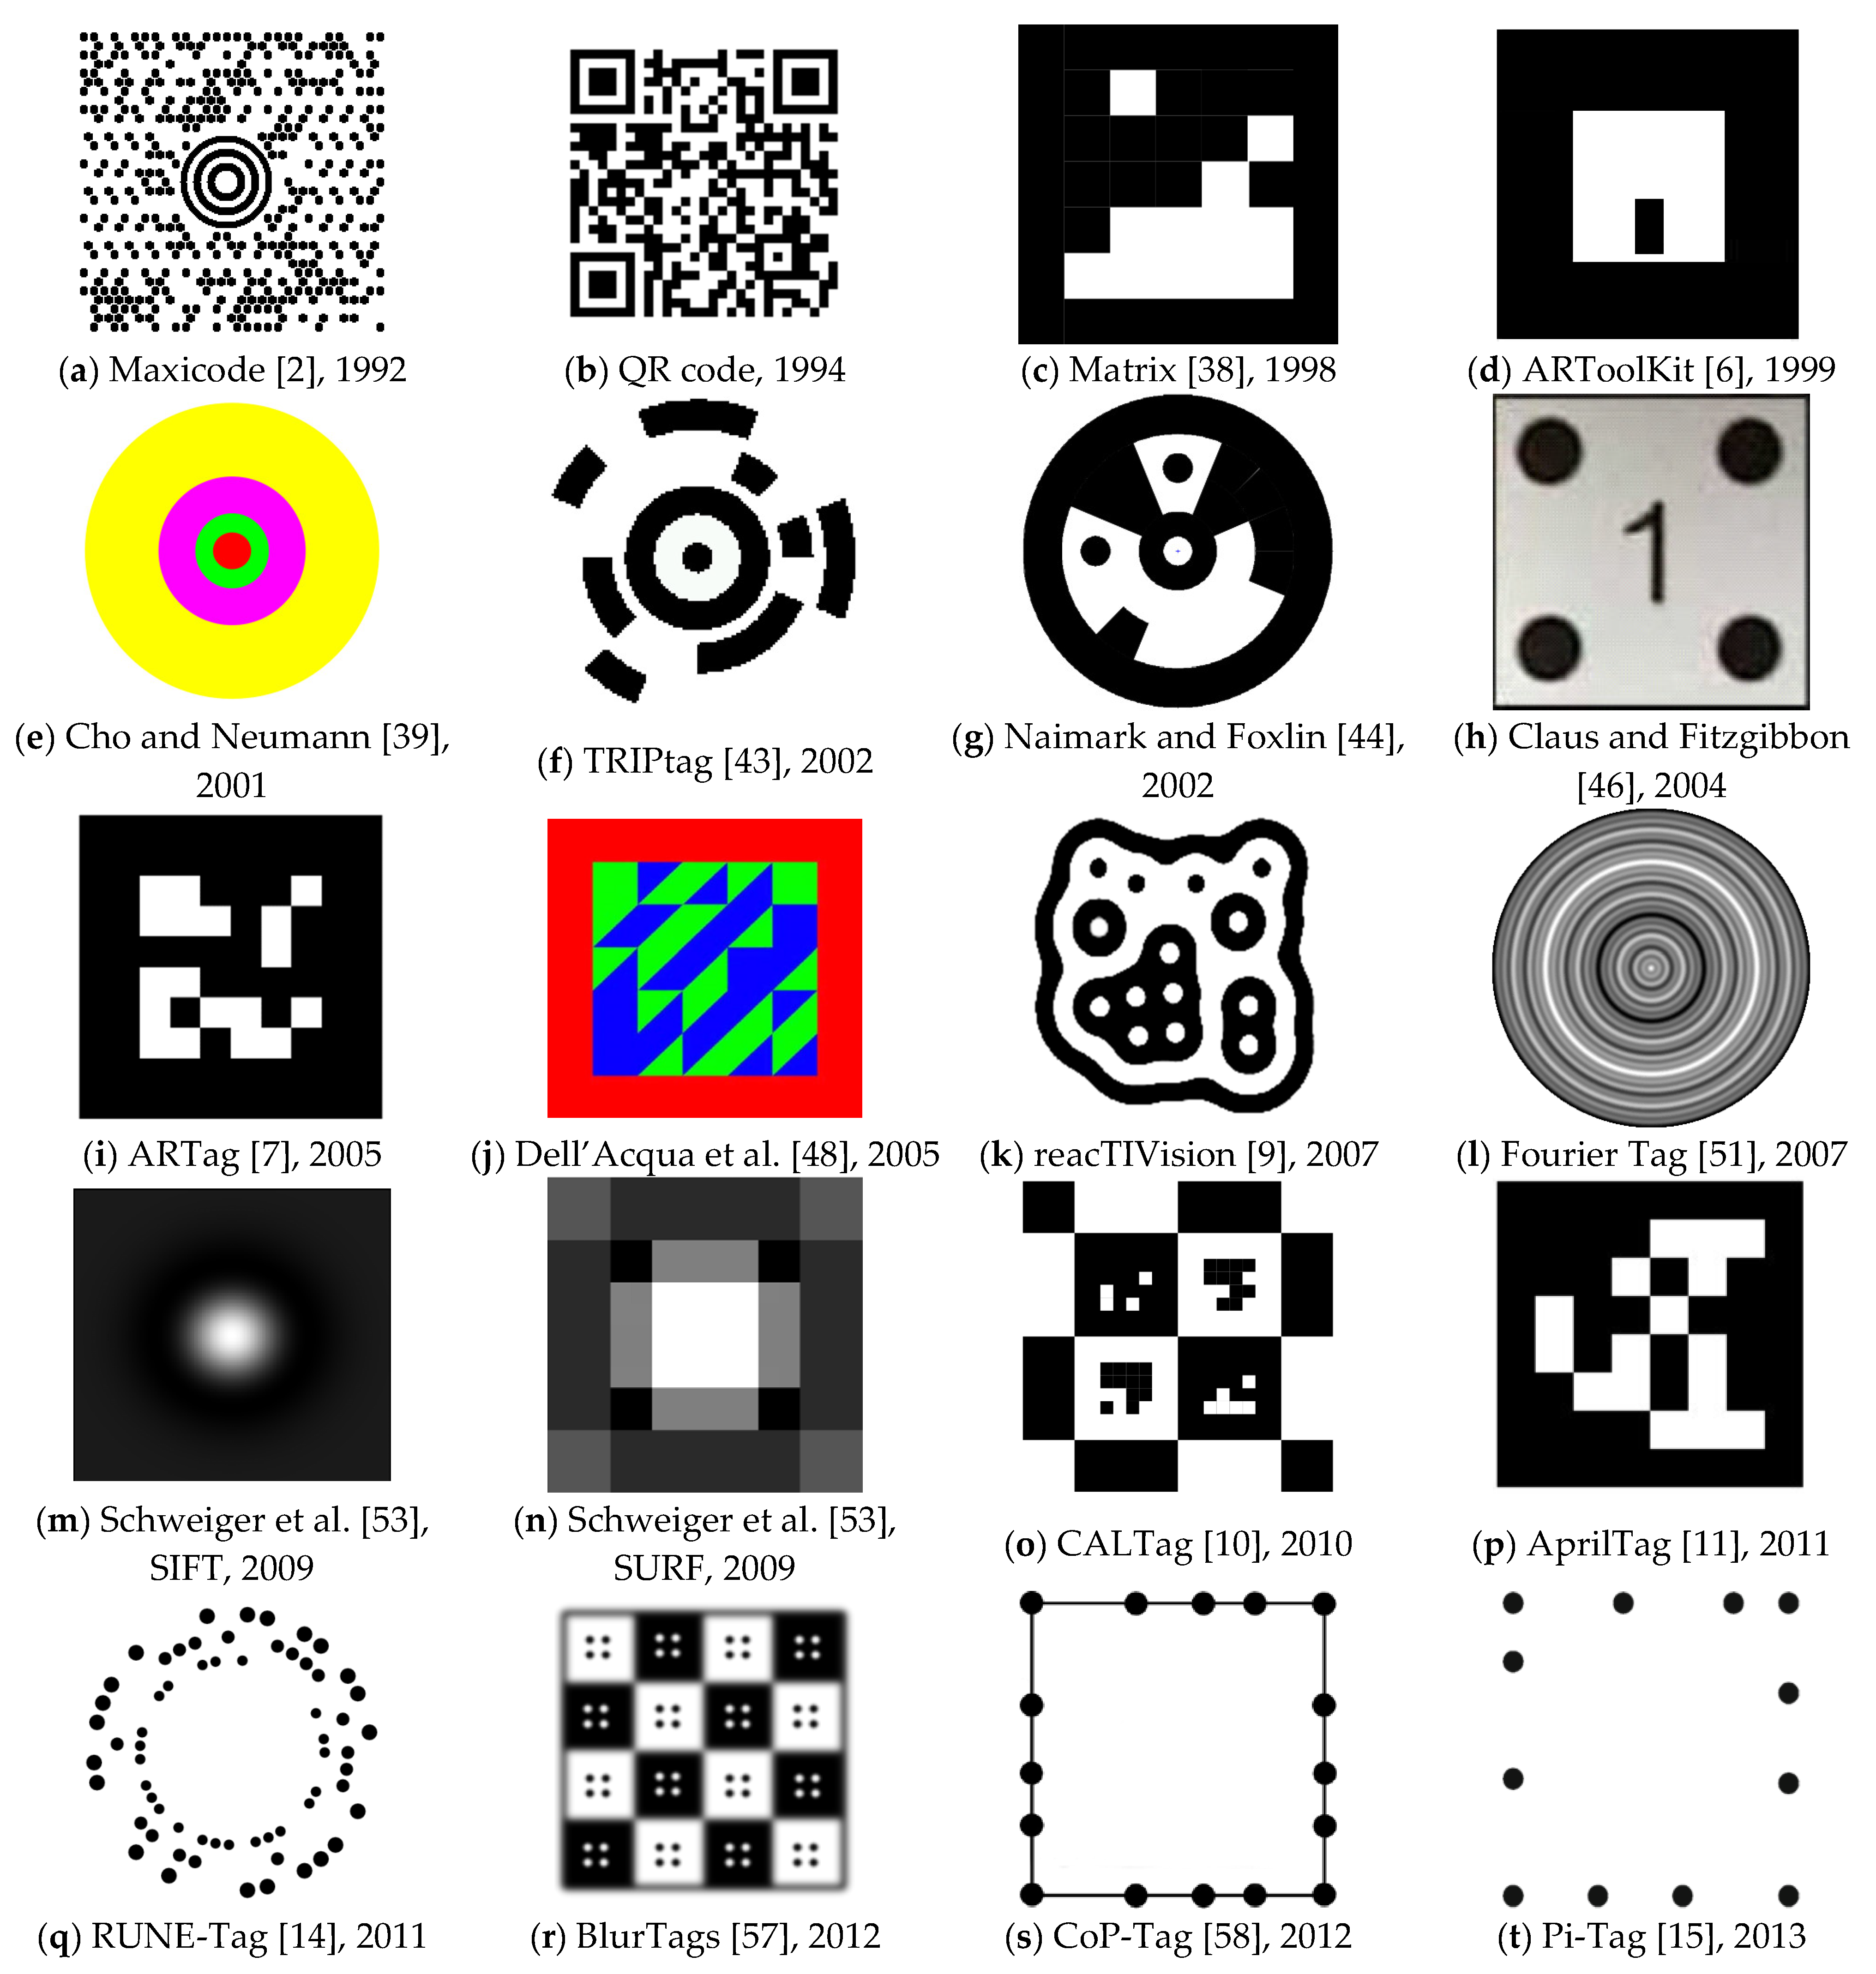
\includegraphics[width=0.8\linewidth]{./figures/fiducialMarkers.png}
	\caption{Marker fiduciari\cite{GARRIDOJURADO20142280}}
	\label{fig:marker_fiduciari}
\end{figure}

\subsection{Applicazioni}
\begin{itemize}
	\item \textbf{Fisica}: per ottenere posizione e riferimenti di oggetti
	\item \textbf{Realtà aumentata}: utilizzo dei marker come ``ancore'' così da sapere dove posizionare gli elementi virtuali nel mondo reale
	\item \textbf{Circuiti stampati}: identificano dei pattern così che i macchinari possano operare sui circuiti in maniera autonoma selezionando i componenti univocamente
	
	
	Vedi video che riporta l'utilizzo di marker fiduciari per un'applicazione di realtà aumentata:
	\href{https://youtu.be/nsu9tNIJ6F0?si=MB4zTZP5yiCO9aW7}{link al video}
\end{itemize}

\subsection{ArUco markers} \label{subsec:aruco_markers}
I marker ArUco sono una tipologia di marker fiduciari binari molto utilizzata in ambiente di visione artificiale.

La caratteristica principale di questo tipo di marker risiede nel fatto di essere estremamente versatile, dove,
con il termine versatile si vuole sottolineare il fatto che questa tipologia di marker non necessita di particolari condizioni di luce ne di grandi capacità di elaborazione per essere processata, in quanto la complessità di ogni marker può variare in base alle esigenze, vedi figura \ref{fig:aruco_marker_0}.

Un altro aspetto fondamentale degli ArUco marker riguarda il fatto che, attraverso sistemi di posa della camera, utilizzata per ottenere le posizioni dei marker, è possibile calcolare anche la loro rotazione.

\subsubsection{Come funzionano?}
All'interno del marker abbiamo dei quadrati bianchi e neri che, in base alla loro disposizione identificano univocamente il marker stesso, il numero di questi quadrati e la loro disposizione possono variare in base al ``dizionario'' selezionato

\subsubsection{Dizionario} \label{subsubsec:dizionario}
\label{Dizionario}
\begin{figure}
	\centering
	
\includegraphics[width=0.5\linewidth]{./figures/4x4_1000-0.png}
	\caption{ArUco Marker 4x4 id: 0}
	\label{fig:aruco_marker_0}
\end{figure}
Ogni ArUco marker appartiene ad un dizionario il quale ne specifica la dimensione e la disposizione interna dei quadrati bianchi e neri, modificando il dizionario possiamo ottenere marker più grandi e complessi che consentono rilevazioni più precise, riducendo la possibilità di confondere tra loro due marker simili, d'altro canto utilizzando marker più piccoli e semplici, nonostante si vada incontro ad una riduzione della precisione, si guadagna in velocità di elaborazione. \cite{reverseEngineeringArucoMarkers}
 
\begin{center}
	\gls{dizionario4x4_100}
\end{center}

\section{OpenCV} \label{sec:opencv}
\acrfull{opencv} è una libreria realizzata inizialmente da Intel pensata per fornire funzioni di visione artificiale che facilitassero il compito degli sviluppatori, garantendo loro un'infrastruttura stabile sulla quale poter sviluppare \ref{fig:opencvLogo}.
\begin{figure}
	\centering
	
\includegraphics[width=0.3\linewidth]{figures/opencvLogo.png}
	\caption{logo OpenCV}
	\label{fig:opencvLogo}
\end{figure}


OpenCV è una libreria multi-piattaforma rilasciata su una licenza open-source, questo ha portato durante gli anni ad una crescita continua grazie anche all'aiuto della community, che ha permesso alla libreria in questione di diventare una tra le più importanti nel suo ambito. \cite{baggio2015opencv} \cite{OpenCVMainPage}

\subsection{JavaCV} \label{subsec:javacv}
JavaCV è un wrapper per la libreria OpenCV, in grado di fornire, oltre a tutte le funzionalità di OpenCV, anche molti metodi per processare immagini e video, questo fa si che con una singola dipendenza si sia in grado di utilizzare tutte le funzionalità in maniera agevolata attraverso il wrapper, senza dover interagire con il codice nativo di OpenCV \cite{javaCVRepo}

\section{Aggregate Computing}
Prima di poterci addentrare nel concetto di aggregate computing è importante spendere due parole per introdurre i sistemi distribuiti dai quali poi saremo in grado di derivare l'idea alla base dell'aggregate computing.

\subsection{Sistema distribuito}
Un sistema distribuito rappresenta una rete di processi o ``nodi di elaborazione" che svolgono calcoli individualmente ma che appaiono dall'esterno come un unico sistema.

Questo tipo di approccio è caratterizzato da una grande eterogeneità sia a livello hardware che software, la quale porta il sistema ad essere aperto a tecnologie diverse, che comunicano tra loro attraverso lo scambio di messaggi per far apparire il sistema distribuito come un'entità unica.

L'aspetto fondamentale di questi sistemi riguarda il fatto che ad ogni singolo \gls{nodo} viene affidato un compito da espletare, il nodo in questione può comunicare con gli altri al fine di portare a termine il suo compito e può essere a sua volta interrogato dagli altri per fornire i risultati della sua elaborazione.
Tutto questo può essere visto dall'esterno come un unico sistema che però al suo interno è composto da una serie di dispositivi con compiti differenti che contribuiscono al raggiungimento di uno scopo comune \ref{fig:centralizedVsDistributed}
\begin{figure}
	\centering
	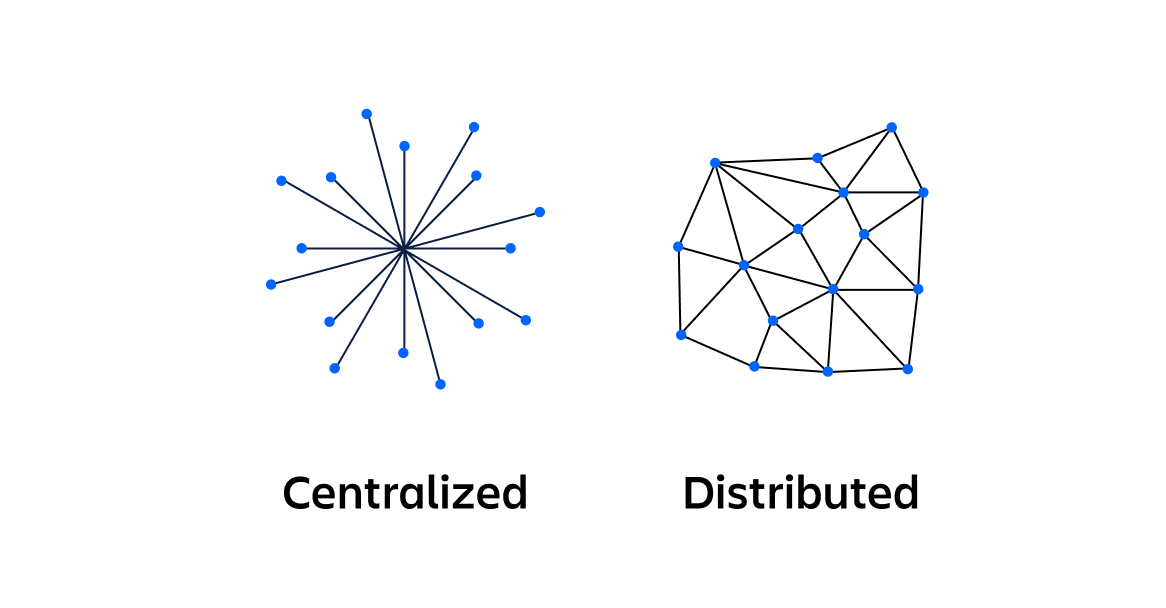
\includegraphics[width=0.8\linewidth]{figures/centralizedVsDistributed.png}
	\caption{Sistema centralizzato Vs distribuito \cite{centralizedVsDistributed}}
	\label{fig:centralizedVsDistributed}
\end{figure}

\subsection{Aggregate computing}
Il termine Aggregate computing rappresenta un approccio emergente nell'ambito della gestione di sistemi distribuiti complessi \cite{VIROLI2019100486} che sposta l'attenzione dal calcolo effettuato da un singolo nodo al far emergere un comportamento globale del sistema sulla base dei calcoli effettuati sui singoli nodi.

A primo avviso la differenza tra i due sembra marginale ma se scendiamo più nel dettaglio possiamo notare che un sistema distribuito focalizza la propria attenzione sulla suddivisione dei compiti ai nodi, che possono comunicare tra loro per ottenere un fine comune mentre un sistema di aggregate computing pone maggiore enfasi sullo scambio di informazioni tra nodi vicini, che, comunicando tra loro, fanno emergere una serie di comportamenti complessi che descrivono il sistema nella sua totalità.
Nel contesto di aggregate computing un nodo non è in grado di comunicare con tutti i nodi, ma solamente con quelli a lui vicini, attraverso i quali può progredire nel suo compito e derivare informazioni sulla rete globale, questo suggerisce quindi che il comportamento generale del sistema visto dall'esterno e guidato da interazioni prettamente locali al suo interno.

La cosa importante da ricordare quando si parla di aggregate computing e che un gruppo di nodi locali che comunicano, con il fine di ottenere una serie di risultati, potrebbe non conoscere l'intero sistema che lo circonda

\subsubsection{Vantaggi}
I vantaggi offerti dall'approccio dell'aggregate computing sono molteplici e spesso dipendono proprio dalla modalità operativa del sistema, in questo caso quindi dalla possibilità di derivare comportamenti emergenti sulla base di interazioni locali:
\begin{itemize}
	\item Scalabilità
	\item Tolleranza ai guasti
	\item Auto-organizzazione
\end{itemize}
Questi vantaggi sono dovuti al fatto che ogni nodo comunica solo con i suoi vicini, di conseguenza non conosce l'intera rete, non è quindi importante che la rete resti invariata perché l'eventuale aggiunta o rimozione di un componente non altera il sistema visto dall'esterno grazie alla capacità dei nodi di riorganizzarsi

\subsubsection{Applicazioni}
Le principali applicazioni di sistemi di aggregate computing possono essere ricercate oggi in ambiti quali:
\begin{itemize}
	\item Reti di sensori
	\item Robotica collettiva
	\item Smart cities
	\item sistemi IoT
\end{itemize}
dove con reti di sensori indichiamo una serie di sensori che vengono utilizzati per monitorare una certa area geografica della quale vogliamo estrarre informazioni in maniera aggregata quali temperatura, pressione atmosferica ecc.


Per robotica collettiva si intende tutta quella serie di applicazioni che consentono a robot e droni di auto-organizzarsi e coordinarsi secondo sciami o schemi predefiniti.


Con smart cities e sistemi IoT invece possiamo riassumere le operazioni volte a gestire l'infrastruttura cittadina come l'illuminazione, il controllo dei semafori e del traffico, ma anche sistemi IoT decentralizzati che interagiscono tra loro per organizzarsi e prendere decisioni in autonomia.


\chapter{Analisi}
Questa tesi si pone l'obiettivo di creare un sistema software sviluppato in java o altro linguaggio che sia in grado di essere eseguito sulla \acrfull{jvm}, con il compito di localizzare e tracciare gli spostamenti di alcuni dispositivi\footnote{oggetti di ogni genere e tipo dei quali si vuole conoscere posizione e rotazione chiamati genericamente dispositivi in questa dissertazione} nel campo visivo di una videocamera.

Per poter analizzare correttamente il sistema in questione è necessario però fare un passo indietro, per introdurre il contesto nel quale dovrà inserirsi:
\begin{adjustwidth}{1cm}{0cm}
l'argomento di questa tesi rappresenta solo un componente di un progetto più complesso, sviluppato dai ricercatori dell'università di Bologna, con l'obiettivo di gestire una serie di dispositivi (robot, droni ecc.), connessi tra loro, secondo il paradigma dell'aggregate computing.
Questo approccio permette ai dispositivi della rete di auto-organizzarsi presentando le caratteristiche tipiche della robotica degli sciami.

Il vincolo riguardante il linguaggio da utilizzare, viene dal fatto che il software attualmente usato dai ricercatori è eseguito dalla JVM e di conseguenza per avere un'interazione più semplice tra i due componenti è importante che anche la parte di visione artificiale sia scritta con un linguaggio compatibile.
\end{adjustwidth}

L'aspetto che ha portato alla stesura di questa tesi, si deve ricercare nel fatto che questo tipo di sistema deve poter funzionare anche in applicazioni indoor, nelle quali, l'utilizzo del GPS per tenere traccia degli spostamenti dei dispositivi è ostacolato da numerosi fattori quali pareti e strutture che possono ostacolarne il segnale.

%PUO DARSI CHE DA QUI IN POI NON VADA BENE PERCHE PARLO DI SOLUZIONI E IN ANALISI DOVREI SOLO DEFINIRE IL PROBLEMA QUINDI POTREI SPOSTARE QUESTA PARTE NEL DESIGN O IMPLEMENTAZIONE E SCRIVERE QUI INVECE COSA DEVO FARE NEL DETTAGLIO CIOE PERCHE STO SVILUPPANDO IL SISTEMA DI VISIONE ARTIFICIALE PER LA NOTTE DEI RICERCATORI E SPIEGARE IN BREVE IL PROGETTO NEL SUO INSIEME

%L'alternativa più ovvia sarebbe sicuramente stata l'impiego di un IPS ``Indoor Positioning System" ma, visti i costi e le complicazioni introdotte da questi tipi di sistemi, per mantenere la soluzione quanto più possibile immediata e soprattutto economica abbiamo deciso di optare per l'utilizzo di un sistema di visione artificiale basato su una videocamera e dei marker fiduciari per identificare gli oggetti
\section{Requisiti funzionali} \label{sec:requisiti_funzionali}
\begin{itemize}
	\item Il sistema deve poter rilevare i dispositivi
	\item Il sistema deve poter calcolare distanza, posizione e angolo di rotazione dei dispositivi rispetto ad un punto fissato nello spazio.
	\item Il sistema dovrà poter essere interrogato per ottenere i risultati computati riguardo il posizionamento dei dispositivi.
\end{itemize}
\section{Requisiti non funzionali} \label{sec:requisiti_non_funzionali}
\begin{itemize}
	\item Il sistema deve poter rilevare i dispositivi ad una distanza di due/tre metri.
	\item Il sistema deve essere sufficientemente reattivo da rilevare e tracciare movimenti repentini da parte dei dispositivi.
	\item Il sistema deve rimanere stabile ed affidabile anche in presenza di condizioni di scarsa illuminazione.
	\item Il sistema deve essere efficiente al punto che il tempo impiegato per stimare la posizione dei dispositivi non influenzi il tempo di esecuzione del software in cui è utilizzato.
	\item Il sistema deve essere sufficientemente preciso da garantire un corretto funzionamento generale, senza incorrere in rilevazioni fuorvianti che porterebbero al crash dello stesso.
\end{itemize}
\section{Requisiti tecnologici}
\begin{itemize}
	\item Il sistema deve essere scritto in java o un linguaggio che sia in grado di essere eseguito dalla JVM.
	\item La videocamera utilizzata per la rilevazione dei dispositivi deve avere una risoluzione minima \gls{FullHD}.
\end{itemize}
\section{Analisi del dominio}
Come già sopracitato, l’oggetto di questa tesi andrà a costituire parte di un sistema più ampio, il quale, una volta assemblato, sarà in grado di:
\begin{enumerate}
	\item \underline{Rilevare e tracciare gli spostamenti dei dispositivi.}
	\item Inviare ai vari nodi le informazioni acquisite durante la fase di rilevazione.
	\item Far comunicare tra loro i nodi vicini.
	\item Far organizzare in maniera autonoma i diversi dispositivi attraverso le informazioni raccolte, secondo algoritmi di aggregate computing senza quindi il bisogno di elaborare gli spostamenti e le nuove posizioni in maniera centralizzata.
\end{enumerate}
\begin{figure}
	\centering
	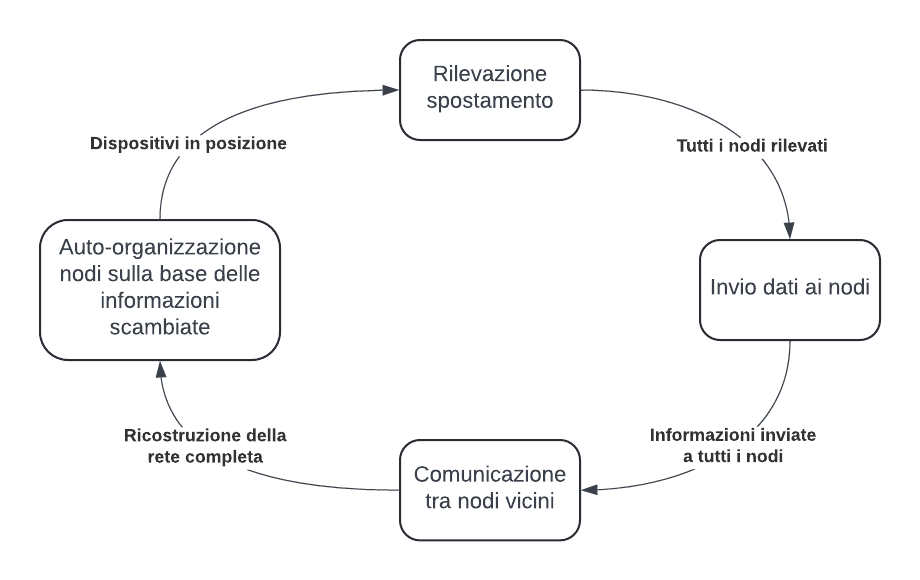
\includegraphics[width=0.8\linewidth]{./figures/UML/domainDiagram.png}
	\caption{Diagramma a stati semplificato del dominio}
	\label{fig:domain_diagram}
\end{figure}
\chapter{Design}
%qui invece devi iniziare a parlare delle soluzioni, scendendo più nel dettaglio e magari mostrando qualche UML ( peccato che io non li abbia :( )
Come già più volte citato, l'ambito di questa tesi è focalizzato sullo sviluppo della componente di visione artificiale utile a rilevare e seguire i dispositivi nel campo visivo della videocamera.

Nelle seguenti sezioni vengono illustrate le scelte, operate in osservanza dei requisiti enunciati nelle sezioni \ref{sec:requisiti_funzionali} e \ref{sec:requisiti_non_funzionali} che costituiranno poi l'implementazione del software oggetto della tesi.

Prima però di poter approfondire l'architettura del sistema è necessario stabilire come rilevare e identificare quelli che finora abbiamo genericamente chiamato ``dispositivi".

\section{ArUco markers}
Dopo un'attenta ricerca volta a determinare quale fosse il metodo più efficacie per poter identificare un qualsiasi oggetto nel campo visivo di una videocamera mi sono imbattuto nei marker ArUco \ref{subsec:aruco_markers}, una tipologia di marker fiduciari \ref{sec:marker_fiduciari} particolarmente utilizzati in contesti di visione artificiale.

La motivazione che mi ha spinto ad utilizzare i marker ArUco deriva dai numerosi vantaggi che questa tecnologia offre, per prima cosa questo tipo di marker è estremamente semplice e scalare, infatti è possibile scegliere fra numerose versioni che si differenziano in base al dizionario utilizzato \ref{subsubsec:dizionario}, inoltre i marker ArUco garantiscono una buona affidabilità anche in condizioni di scarsa illuminazione, scenario da non sottovalutare in una applicazione di visione artificiale, infine un altro vantaggio è sicuramente dato dalla loro velocità di rilevazione che permette quindi l'uso di un gran numero di marker contemporaneamente senza rallentamenti.

Per poter utilizzare i marker ArUco è stata utilizzata la libreria offerta da OpenCV \ref{sec:opencv}

\section{Videocamera}
Per poter rispettare i requisiti imposti in fase di analisi riguardanti la videocamera che il sistema avrebbe utilizzato per ottenere il flusso video, la scelta è ricaduta su una webcam FullHD capace di registrare a 60fps, per contenere i costi, garantire una risoluzione sufficiente al riconoscimento degli oggetti e avere un campo visivo ampio.

\section{Architettura}
Premessa: \textit{L'architettura riguarderà il solo sistema di visione artificiale, realizzato da me come software stand-alone che è poi stato rielaborato dai ricercatori per poterlo integrare con il loro progetto, non verrà trattata l'architettura del sistema finale se non attraverso alcuni cenni utili a comprendere le scelte intraprese.}
\vspace{0.5cm}

\noindent Finora sono state presentate scelte che riguardano la videocamera e l'utilizzo di marker ArUco per rilevare e identificare gli oggetti nella \gls{scena}, dal punto di vista del software invece per ottenere risultati conformi ai requisiti e di conseguenza un sistema capace di operare anche in condizioni di scarsa luminosità, con un buon livello di precisione e a distanze considerevoli, si è reso necessario l'impiego di sistemi di calibrazione della videocamera oltre che ovviamente a funzionalità per determinare la posizione degli oggetti.

Il software da me realizzato si compone di tre parti principali descritte da tre classi java:
\begin{itemize}
	\item App.java
	\item CameraCalibrator.java
	\item CameraPose.java
\end{itemize}
App.java si occupa di orchestrare le diverse fasi di avvio dell'applicazione, consentendo in una fase iniziale di calibrare la camera attualmente in uso attraverso la classe CameraCalibrator.java e in un secondo momento di calcolare la posa della camera rispetto ai marker sulla scena con la classe CameraPose.java. \ref{fig:architettura}
\begin{figure}
	\centering
	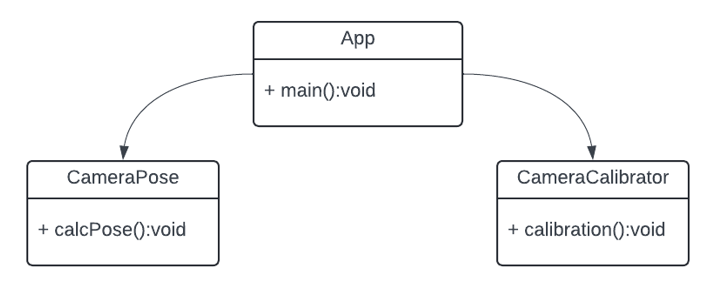
\includegraphics[width=0.8\linewidth]{./figures/UML/architecture.png}
	\caption{Architettura del sistema}
	\label{fig:architettura}
\end{figure}5

%Dovrai dire che l'architettura qui riguarda il solo sistema di visione artificiale come stand-alone e che quindi l'architettura del sistema finale sviluppato dai ricercatori non viene introdotta ne menzionata di seguito
%provvisorio: nell'architettura generale dovrai dire che il sistema si comporrà di tre parti principali, il main che gestirà le varie componenti, del sistema, una parte di calibrazione e una parte di posa e rilevazione.

\section{Design dettagliato}
Entrando più nel dettaglio dell'architettura, il sistema si compone anche di altre due classi denominate: ResolutionEnum.java e InputParameters.java andando quindi a definire il sistema nella sua totalità come in figura: \ref{fig:architettura_completa}
dove le due classi sono rispettivamente una enum che racchiude tutte \footnote{sono riportate solo le risoluzioni più comuni} le risoluzioni che la camera può utilizzare ed una \acrfull{gui} che permette all'utente di configurare il software in base alle proprie preferenze.
\begin{figure}
	\centering
	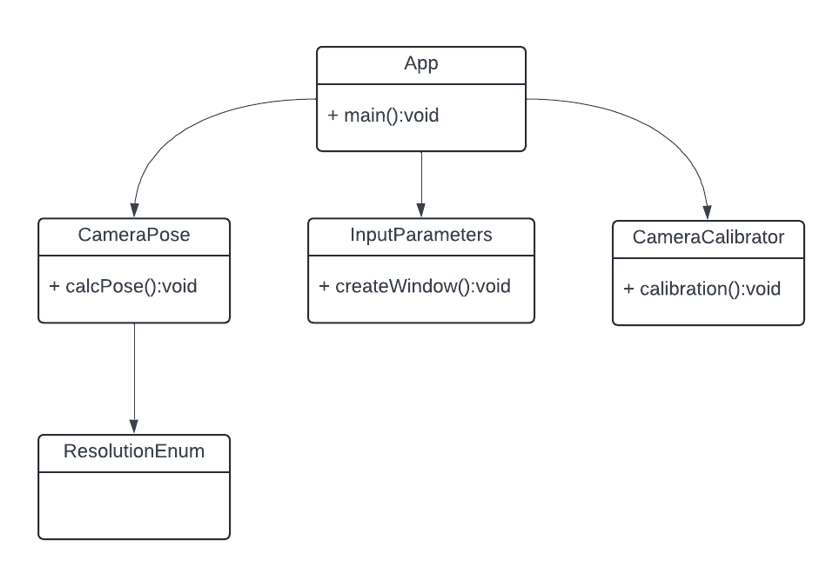
\includegraphics[width=0.8\linewidth]{./figures/UML/fullArchitecture.png}
	\caption{Architettura completa}
	\label{fig:architettura_completa}
\end{figure}
%descrivi precisamente ogni blocco di cui hai fatto lo screen, senza entrare in specifiche di codice e implementazione, potrei anche aggiungere un diagramma a stati che definisce come le varie classi interagiscono tra loro
\subsection{App}
Questa classe rappresenta il punto di ingresso dell'applicazione e si occupa di istanziare tutte le classi necessarie per il corretto funzionamento del sistema all'interno del main. \ref{fig:app}
\begin{figure}
	\centering
	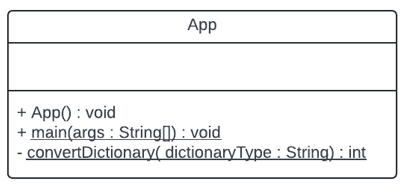
\includegraphics[width=0.5\linewidth]{./figures/UML/app.png}
	\caption{Classe App.java}
	\label{fig:app}
\end{figure}
\subsection{cameraCalibrator}
La classe cameraCalibrator ricopre un ruolo molto importante, il suo obiettivo è quello di calibrare la camera affinché le immagini ottenute consentano di stabilire correttamente la posizione della stessa rispetto agli oggetti nella scena. \ref{fig:camera_calibrator}.

\vspace{0.5cm}
\textit{Di seguito sono riportate alcune informazioni di base per comprendere il concetto di calibrazione della camera}	
\subsubsection{Cos'è la calibrazione?}
La calibrazione è un processo volto a ottenere i parametri della lente e del sensore della videocamera/fotocamera,
tali parametri potranno poi essere impiegati per correggere la distorsione della lente, calcolare distanze, ricostruire l'immagine 3D di partenza ecc \cite{cameraCalibrationMathWorks}.
\subsubsection{Modello di calibrazione}
Esistono diversi modelli di calibrazione in base al tipo di camera che si intende utilizzare, nel nostro caso, ipotizzando l'utilizzo di una webcam, il modello che meglio si adatta è quello di una fotocamera con obiettivo stenopeico \ref{fig:pinhole_camera}, nella quale però teniamo conto anche della distorsione della lente. \cite{pinholeCamera} \cite{pinholeCameraModel} 
\begin{figure}
	\centering
	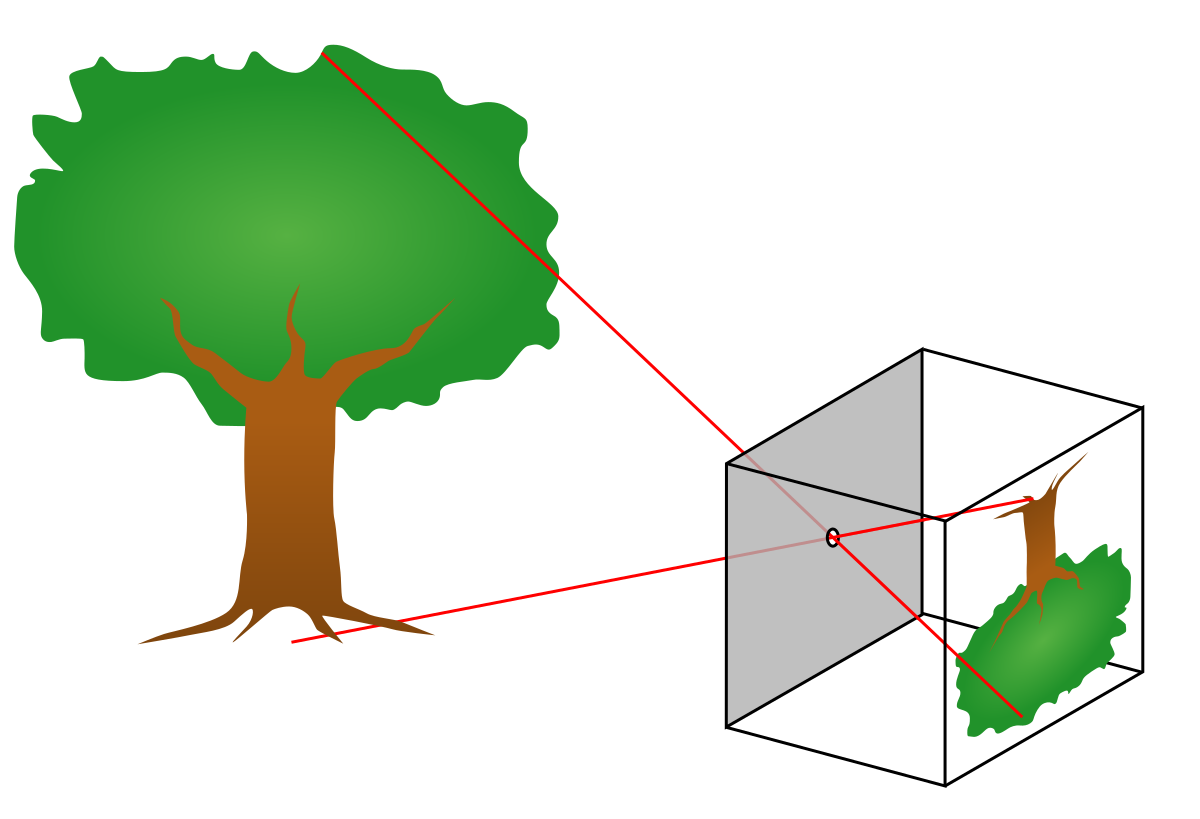
\includegraphics[width=0.5\linewidth]{./figures/Pinhole-camera.png}
	\caption{Rappresentazione camera con obiettivo stenopeico}
	\label{fig:pinhole_camera}
\end{figure}

Il parametro più importante è la matrice della camera ``camera matrix" che mappa le coordinate del mondo 3D nell'immagine 2D catturata, questa matrice è ottenuta a partire dai parametri intrinseci e estrinseci:
\begin{itemize}
	\item Parametri estrinseci: rappresentano la posizione e rotazione della camera nel mondo reale.
	\item Parametri intrinseci: consentono di trasformare le coordinate della camera 3D nelle coordinate dell'immagine 2D.
\end{itemize}
l'obiettivo della calibrazione è proprio quello di determinare questi due parametri così da poter calcolare la matrice della camera. \ref{fig:calibration_cameramodel_coords}
\begin{figure}
	\centering
	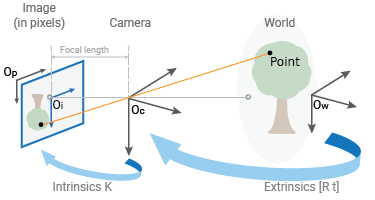
\includegraphics[width=0.5\linewidth]{./figures/calibration-cameramodel-coords.png}
	\caption{Processo di conversione dal mondo reale 3D all'immagine 2D}
	\label{fig:calibration_cameramodel_coords}
\end{figure}

\subsubsection{Distorsione della lente}
Un altro aspetto fondamentale da tenere in considerazione riguarda la distorsione introdotta dalla lente della camera, nel modello utilizzato infatti si trascura l'uso della lente ma in situazioni reali l'obiettivo gioca un ruolo cruciale, poiché introduce due tipi di distorsione:
\begin{itemize}
	\item Distorsione radiale: condizione per la quale i raggi di luce vengono curvati in maniera non uniforme, deformando l'immagine finale a partire dal centro dell'obiettivo. \ref{fig:radial_distortion}
	\begin{figure}
		\centering
		
\includegraphics[width=0.5\linewidth]{./figures/radial_distortion.png}
		\caption{Distorsione radiale}
		\label{fig:radial_distortion}
	\end{figure}
	\item  Distorsione tangenziale: distorsione che ha luogo nel caso in cui la lente è il piano che si vuole fotografare non sono paralleli. \ref{fig:tangential_distortion}
	\begin{figure}
		\centering
		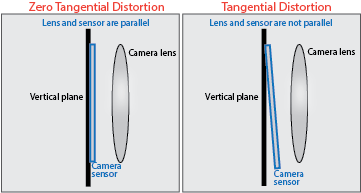
\includegraphics[width=0.5\linewidth]{./figures/tangential_distortion.png}
		\caption{Distorsione tangenziale}
		\label{fig:tangential_distortion}
	\end{figure}
\end{itemize} 
\begin{figure}
	\centering
	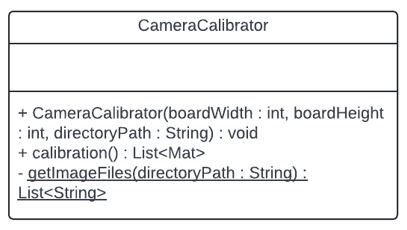
\includegraphics[width=0.5\linewidth]{./figures/UML/cameraCalibrator.png}
	\caption{Classe CameraCalibrator.java}
	\label{fig:camera_calibrator}
\end{figure}
\subsection{cameraPose}
La classe CameraPose rappresenta il fulcro del progetto, grazie ai metodi sviluppati è possibile ottenere la posa della camera rispetto agli oggetti identificati dai marker ArUco. Le informazioni ricavabili riguardano distanza, posizione e rotazione dei marker, inoltre è anche possibile visualizzarne graficamente lo spostamento e l'orientamento. \ref{fig:camera_pose}
\begin{figure}
	\centering
	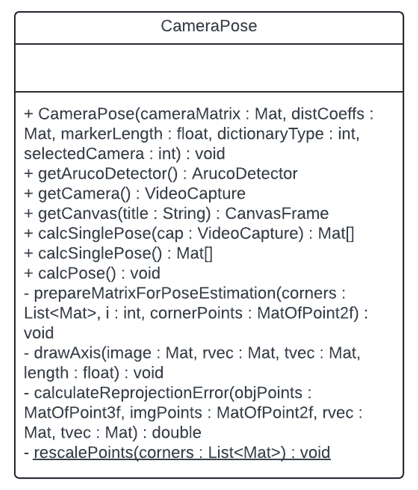
\includegraphics[width=0.5\linewidth]{./figures/UML/cameraPose.png}
	\caption{Classe CameraPose.java}
	\label{fig:camera_pose}
\end{figure}
\subsection{resolutionEnum}
Enumerazione in grado di fornire i formati più utilizzati per flussi video. \ref{fig:resolution_enum}
\begin{figure}
	\centering
	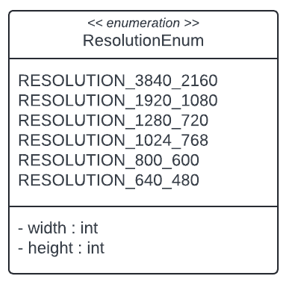
\includegraphics[width=0.5\linewidth]{./figures/UML/resolutionEnum.png}
	\caption{Classe ResolutionEnum.java}
	\label{fig:resolution_enum}
\end{figure}
\subsection{inputParameters}
La classe InputParameters rappresenta una GUI con la quale l'utente finale può interagire, al fine di configurare il programma in base alle proprie specifiche e preferenze. \ref{fig:input_parameters}
\begin{figure}
	\centering
	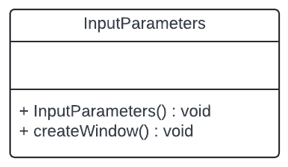
\includegraphics[width=0.5\linewidth]{./figures/UML/inputParameters.png}
	\caption{Classe InputParameters.java}
	\label{fig:input_parameters}
\end{figure}
\subsection{cameraPoseBlock}
Nell'immagine \ref{fig:camera_pose_block} viene mostrata l'associazione tra la classe CameraPose.java e la classe ResolutionEnum.java, grazie alla quale la prima riesce ad ottenere l'elenco delle possibili risoluzioni video utilizzate dalla camera.
\begin{figure}
	\centering
	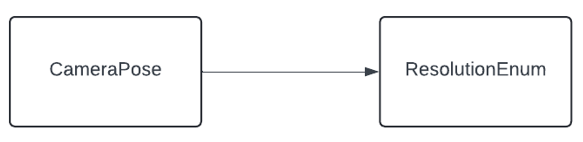
\includegraphics[width=0.5\linewidth]{./figures/UML/cameraPoseBlock.png}
	\caption{Associazione ResolutionEnum.java}
	\label{fig:camera_pose_block}
\end{figure}
\subsection{UI}
Nell'associazione in figura \ref{fig:UI} App.java fa uso della classe InputParameters.java per poter istanziare correttamente i parametri utili al software per adattarsi all'ambiente in cui il sistema viene impiegato.
\begin{figure}
	\centering
	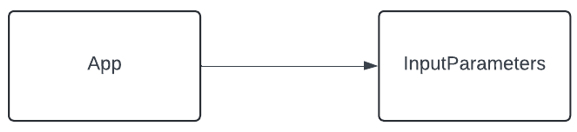
\includegraphics[width=0.5\linewidth]{./figures/UML/UI.png}
	\caption{Associazione InputParameters.java}
	\label{fig:UI}
\end{figure}

%provvisorio: nel design dettagliato procederai a definire un po' più nel dettaglio le tre componenti enunciate nell'architettura senza entrare troppo nello specifico dell'implementazione ma limitandoti a definire i compiti delle tre parti

\chapter{Implementazione}
%descrivi le varie fasi di calibrazione posa ecc. riferendoti a quanto già espresso durante la fase di analisi e soprattutto design

%dovrai parlare meglio anche delle funzioni di openCv dato che nel design hai appena accennato a OpenCV
%vedi tu se inserire i calcoli matematici presenti anche nella pagina di opencv per la calibrazione e posa degli ArUco marker, utili a stimare parametri intrinsechi e estrinsechi della camera e la posa
\chapter{Valutazione}

\chapter{Conclusioni}

\chapter{Sviluppi futuri}

\chapter{Ringraziamenti}

I suggest referencing stuff as follows: \cref{fig:random-image} or \Cref{fig:random-image}

\begin{figure}
    \centering
    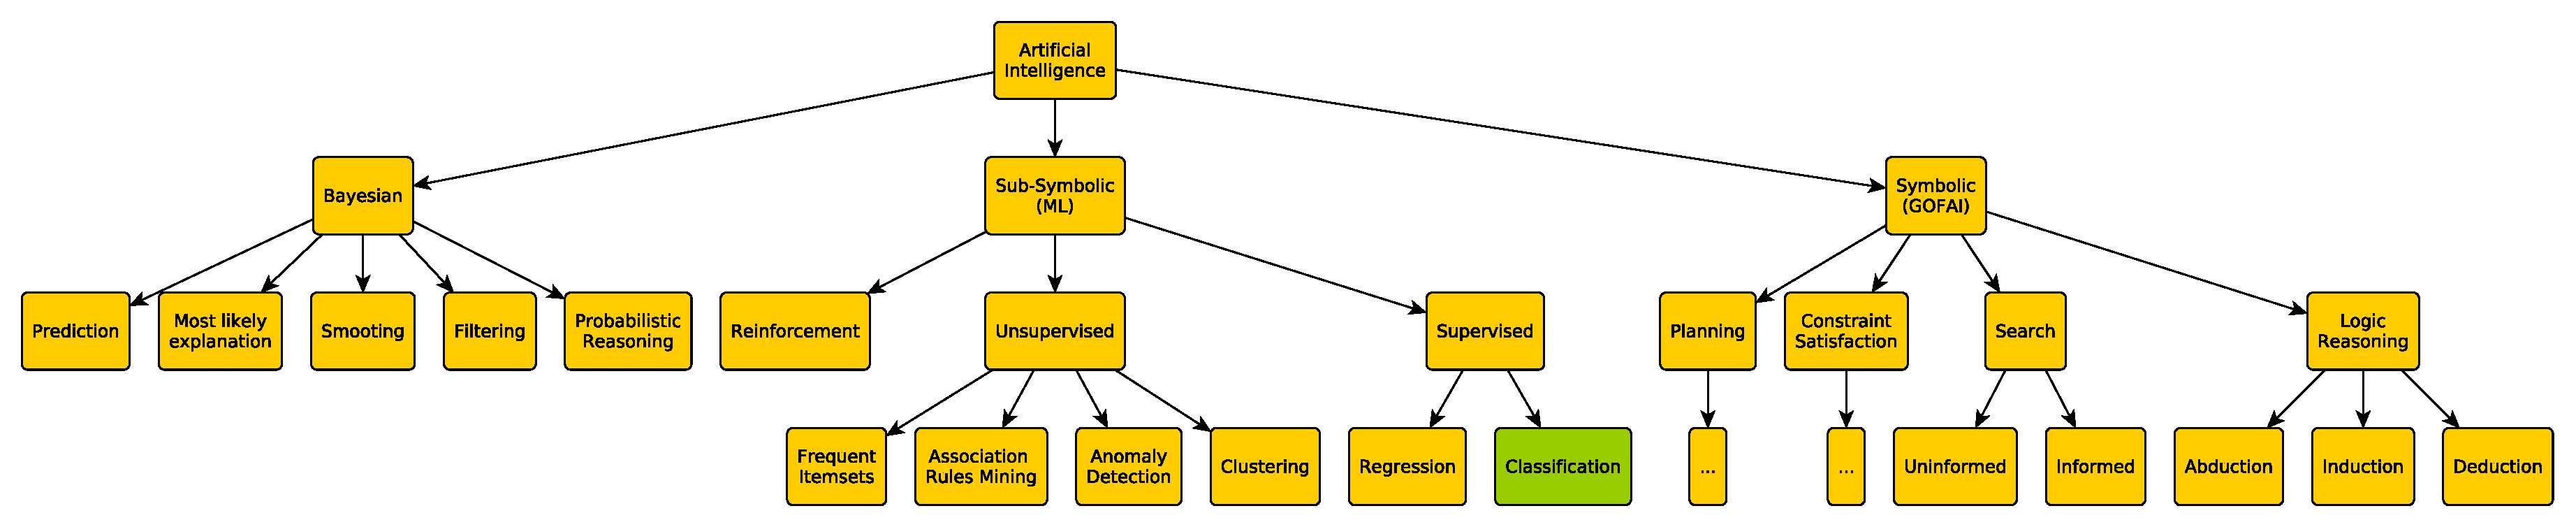
\includegraphics[width=0.8\linewidth]{figures/random-image.pdf}
    \caption{Some random image}
    \label{fig:random-image}
\end{figure}

\section{Some cool topic}

\chapter{Contribution}

You may also put some code snippet (which is NOT float by default), eg: \cref{lst:random-code}.

\lstinputlisting[float,language=Java,label={lst:random-code}]{listings/HelloWorld.java}

\section{Fancy formulas here}

%----------------------------------------------------------------------------------------
% BIBLIOGRAPHY
%----------------------------------------------------------------------------------------

\backmatter

\nocite{*} % Remove this as soon as you have the first citation
\printglossary[type=\acronymtype]
\printglossary
\printbibliography

\begin{acknowledgements} % this is optional
Optional. Max 1 page.
\end{acknowledgements}

\end{document}
